

\documentclass{article}
\title{Bounding parameter uncertainty in single molecule localization}
\author{C.W. Seitz}
\date{\today}

\usepackage{graphicx}
\usepackage{subfigure,epsfig,amsfonts}
\usepackage{amsmath}
\usepackage{siunitx}
\usepackage{float}
\usepackage{bm}
\usepackage{natbib}
\bibliographystyle{unsrtnat}

\begin{document}
\maketitle

\section{An ideal single element detector}

Suppose that we have an imaginary single element detector $k$, with a magical shape, that has the potential to detect every photon emitted by a fluorophore. The fluorophore emits photons according to a Poisson process with rate $\eta$, which can be shown to have mean $\mu = \eta\Delta t$ where $\Delta t$ is the exposure time. The only source of photon-loss, is the quantum efficiency of $k$, which is a probability $0 \leq \gamma \leq 1$ that a photon is detected. We then have two random variables at play (1) how many photons will be emitted in $\Delta t$ and (2) whether not each photon emitted will be detected:

\begin{equation*}
M_{k} \sim \mathrm{Poisson}(\eta)\hspace{0.2in}N_{k} \sim \mathrm{Bern}(\gamma, 1-\gamma)
\end{equation*}

As mentioned, the probability $M_{k}$ photons will be detected in the exposure time $\Delta t$ is is a discrete Poisson random variable, which has the form 

\begin{equation*}
\mathrm{Poisson}(n; \eta) = \frac{\exp\left({-\eta\Delta t}\right)(\eta\Delta t)^{n}}{n!}
\end{equation*}

Based on our intuition, we might expect that throwing out each photon with probability $\gamma$ will effectively reduce the rate of the Poisson process by a factor of $\gamma$. However, we would like to prove this in a mathematically rigorous way. We start by noting that we can define a new variable $S_{k} = M_{k}N_{k}$ such that our measurment is sampled from the density $P(S_{k})$. Let's write the joint distribution over all three variables

\begin{align*}
P(S_{k},M_{k},N_{k}) &= P(S_{k}|M_{k}=m_{k},N_{k}=n_{k})P(M_{k}|N_{k}=n_{k})P(N_{k}=n_{k})
\end{align*}

Note that $m_{k},s_{k} \in \Omega$ where $\Omega = \{z \in \mathbb{Z}: z \geq 0\}$ We can marginalize this distribution over $M_{k}$ and $N_{k}$

\begin{align*}
P(S_{k})  &= \sum_{m_{k}}\sum_{n_{k}} P(S_{k}|M_{k}=m_{k},N_{k}=n_{k})P(M_{k}|N_{k}n_{k})P(N_{k}=n_{k})
\end{align*}

Expanding this expression out over the support of $N_{k}$ gives

\begin{align*}
P(S_{k}) &= \sum_{m_{k}}P(S_{k}|M_{k}=m_{k},N_{k}=0)P(M_{k}|N_{k}=0)P(N_{k}=0)\\
&+ P(S_{k}|M_{k}=m_{k},N_{k}=1)P(M_{k}|N_{k}=1)P(N_{k}=1)
\end{align*}

At this point it is quite clear that we have

\begin{align*}
P(S_{k}) &= \sum_{m_{k}}\gamma\delta(s_{k}-m_{k})P(M_{k}=m_{k})+(1-\gamma)\delta(s_{k}) P(M_{k}=m_{k})\\
&= \gamma P(M_{k}) + \delta(s_{k})(1-\gamma)
\end{align*}

Interestingly, this result is fairly intuitive - the distribution $P(S_{k})$ is given by multiplying the probability mass $P(M_{k})$ by a factor of $\gamma$ and inflating the value at zero by the difference between the new and old distributions. It is worth nothing that adding $1-\gamma$ to the probability mass at zero is effectively reducing the Poisson rate $\eta$ to $\gamma\eta$, since the probability of observing an event is uniform in the interval $(t, t+\Delta t)$. Therefore, we conclude that

\begin{align*}
P(S_{k}) &= \mathrm{Poisson}(S_{k}; \lambda_{k})
\end{align*}

where we have used the \emph{effective rate} $\lambda_{k} = \gamma\eta_{k}$. 

\subsection{Corrupting the signal}

In the real-world, noise is unavoidable. Detectors often suffer from dark noise (thermal noise) and there may also be a background signal. Considering the former first, we define another r.v. $W_{\theta,k}$ which represents Gaussian dark noise of the detector element. Unless otherwise specified we will always assume that $W_{k} \sim \mathcal{N}(m_{k},\sigma_{w,k}^{2})$. Adding in dark noise leads to yet another distribution, this time over the corrupted signal $H_{k}$. Notice that while $S_{k}$ has units of photons $[\mathrm{p}]$, that $H_{k}$ has units of photoelectrons $[e^{-}]$. The conversion factor between the two is the gain of the detector element $g_{k}\; [e^{-}\mathrm{p}^{-1}]$. Moving on, we employ a similar trick as before, evaluating the joint density $P(S_{k},H_{k})$

\vspace{0.1in}
\begin{align*}
P(S_{k},H_{k}) &= P(H_{k}|S_{k})P(S_{k})\\
&= \frac{1}{Z}\exp\left(-\frac{(H_{k}-g_{k}n_{k})^{2}}{\sigma_{k}^{2}}\right)\frac{\exp\left({-\lambda_{k}}\right)\lambda_{k}^{n_{k}}}{n_{k}!}
\end{align*}
\vspace{0.1in}

Marginalizing over $S_{k}$ gives the desired distribution over $H_{n}$

\begin{equation*}
P(H_{k}) = \frac{1}{Z}\sum_{n_{k}=0}^{\infty}\frac{\exp\left({-\lambda_{k}}\right)\lambda_{k}^{n_{k}}}{n_{k}!}\exp\left(-\frac{(H_{k}-g_{k}n_{k})^{2}}{\sigma_{k}^{2}}\right)
\end{equation*}

\begin{figure}
\centering     %%% not \center
\subfigure[Theoretical prediction of $P(S_{k},H_{k})$ and marginal distributions for $g_{k}=1$, $\lambda_{k}=10\;\mathrm{cpms}$, and $\Delta t = 5\si{ms}$ and $\sigma_{k}=5 \;e^{-}$]{\label{fig:a}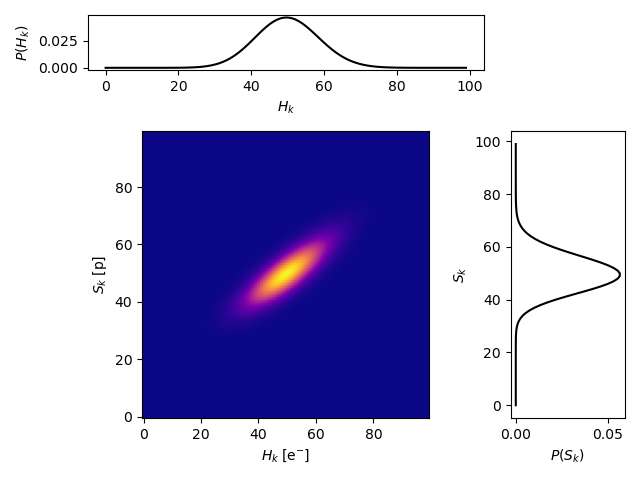
\includegraphics[width=120mm]{theoretical}}
\subfigure[Simulation of $P(S_{k},H_{k})$ and marginal distributions]{\label{fig:b}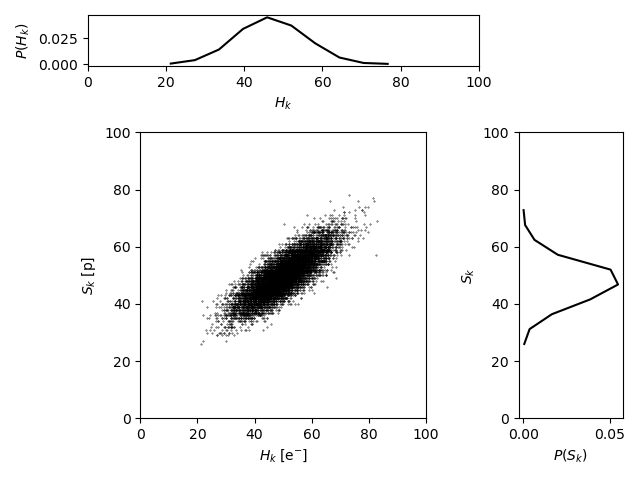
\includegraphics[width=120mm]{experimental}}

\end{figure}

Notice that when $\mu_{k} = \lambda_{k}\Delta t$ is large, $P(S_{k})$ is well-approximated by a Gaussian distribution. It turns out the for $\mu > 20$ the Poisson distribution is approximately 

\begin{equation*}
S_{k} \sim \mathcal{N}(\lambda_{k}\Delta t, \lambda_{k}\Delta t)
\end{equation*} 

which turns out to be a very useful approximation for simplifying $P(H_{k})$. It can be shown that the product of two Gaussian PDFs is

\begin{equation*}
\mathcal{N}(\mu_{1},\sigma_{1}^{2}) \times \mathcal{N}(\mu_{2},\sigma_{2}^{2}) = \mathcal{N}\left(\frac{\mu_{1}\sigma_{2}^{2} + \mu_{2}\sigma_{2}^{2}}{\sigma_{1}^{2}+\sigma_{2}^{2}}, \frac{1}{\frac{1}{\sigma_{1}^{2}}+\frac{1}{\sigma_{2}^{2}}}\right)
\end{equation*}

a property which we can apply to the above equation to get

\begin{equation*}
P(H_{k}) = \frac{1}{Z}\sum_{n_{k}=0}^{\infty}\exp\left(-\frac{1}{2}\left(H_{k}-\frac{g_{k}n_{k}(\lambda_{k}\Delta t)^{2} +  (\lambda_{k}\Delta t)\sigma_{k}^{2}}{(\lambda_{k}\Delta t)^{2}+\sigma_{k}^{2}}\right)\left(\frac{1}{(\lambda_{k}\Delta t)^{2}}+\frac{1}{\sigma_{k}^{2}}\right)\right)
\end{equation*}

\section{An array detector}

Most detectors used for imaging have many elements (pixels) so that we can record an image projected onto the detect by a lens or system of lenses. Due to diffraction, a point emitter will be registered as a diffraction limited spot. We will adopt the Gaussian PSF approximation for such a spot:

\begin{equation*}
q(x,y) = \frac{1}{2\pi\sigma^{2}}\exp\left(-\frac{(x-x_{0})^{2}+(y-y_{0})^{2}}{2\sigma^{2}}\right)
\end{equation*}

The function $q(x,y)$ can be thought of an the intensity profile of the fluorophore emission, although this is not exactly correct. The wave particle-duality in quantum mechanics says that observation of a wave produces a particle, and our detector is nothing but an observer. The EM field that is waving is observed and then we record a particle. However, the statistical nature of quantum mechanics says that $q(x,y)$ is actually a probability distribution and our photons are samples from it. The detector array is binning those samples in a 2D histogram that we call an image. All that said, the Poisson rate at every pixel is not the same and we need to re-evaluate $P(S_{k})$ for each pixel. This is fairly simple, since the rate at every bin is just the probability assigned to that bin, which is an integral of $q(x,y)$ over the bin

\begin{equation*}
\lambda_{k} = \gamma\cdot\int_{C_{k}} q(x,y)dxdy
\end{equation*}

\section{Fisher information and the Cramer-Rao bound}

\subsection{Example: Fisher information for the normal distribution}

Suppose the we have a normally distributed random variable $X \sim \mathcal{N}(\mu,\sigma^{2})$ where $\mu$ and $\sigma^{2}$ are both unknown parameters. We are also given a batch of $N$ samples $\{X_{i}\}_{i=1}^{N}$ and we would like to know how much information those samples carry about our parameters $\theta = (\mu,\sigma)$. In principle there is some probability distribution $P(\theta)=P(\mu,\sigma)$ which can be initially taken to be uniform (which has maximum entropy). A natural question that follows is, how much does the batch of samples reduce the entropy of $P(\theta)$ and thus our uncertainty about $\theta$?

\begin{align*}
I_{ij}(\theta) = \underset{{x\sim p}}{\mathbb{E}}\left[\frac{\partial}{\partial\theta_{i}} \left(\ell(x|\theta)\right)\frac{\partial}{\partial\theta_{j}} \left(\ell(x|\theta)\right)\right]
\end{align*}

For the 1D normal distribution, we only have two parameters, so the Fisher information matrix has a simple form 

\begin{align*}
\mathbf{I}(\theta) = \begin{pmatrix}
\partial_{\mu}^{2}\ell & \partial_{\mu}\partial_{\sigma} \\
\partial_{\sigma}\partial_{\mu} & \partial_{\sigma}^{2}\ell
\end{pmatrix}
\end{align*}

It is straightforward to show that the log-likelihood of the data for this model is given by

\begin{align*}
\ell(x|\theta) = -\frac{1}{2}\log 2\pi\sigma^{2} - \frac{(x-\mu)^{2}}{2\sigma^{2}}
\end{align*}

\begin{align*}
\partial_{\mu}^{2}\ell = -\partial_{\mu}^{2}\frac{(x-\mu)^{2}}{2\sigma^{2}}
\end{align*}

\subsection{The array detector again}

When there are many parameters, the Fisher Information (second moment of the score) is a covariance matrix

\begin{align*}
I_{ij}(\theta) = \underset{{x\sim p}}{\mathbb{E}}\left[\frac{\partial}{\partial\theta_{i}} \left(\ell(x|\theta)\right)\frac{\partial}{\partial\theta_{j}} \left(\ell(x|\theta)\right)\right]
\end{align*}

We have shown that the model for the number of photoelectrons at a pixel is

\begin{equation*}
P(H_{k}) = \frac{1}{Z}\sum_{s=0}^{\infty}\frac{\exp\left({-\lambda_{k}}\right)\lambda_{k}^{n_{k}}}{n_{k}!}\exp\left(-\frac{(H_{k}-g_{k}n_{k})^{2}}{\sigma_{k}^{2}}\right)
\end{equation*}

As we have noted above, $\lambda_{k}$ is dependent on $\int q(x,y)dxdy$ and therefore the PSF parameters $\theta = (\mu_{x},\mu_{y},\sigma)$. These can be plugged into the following Fisher information matrix

\begin{align*}
I_{ij}(\theta) &= \underset{{H\sim P(H)}}{\mathbb{E}}\left[\frac{\partial}{\partial\theta_{i}} \log P(H_{k})\frac{\partial}{\partial\theta_{j}} \log P(H_{k})\right]\\
&= \underset{{H\sim P(H)}}{\mathbb{E}}\left[\frac{\partial}{\partial\theta_{i}} \log P(H_{k})\frac{\partial}{\partial\theta_{j}}\log P(H_{k})\right]
\end{align*}

where $H\sim P(H)$ is perhaps a small patch of an image containing a diffraction limited spot. We need to then calculate the derivatives with respect to each of the parameters $\theta = (x_{0},y_{0},\sigma)$. 

\begin{align*}
\frac{\partial}{\partial x_{0}}\log P(H_{k}) &= \frac{1}{P(H_{k})} \frac{\partial P(H_{k})}{\partial x_{0}}\\
&=  \frac{1}{ZP(H_{k})}\sum_{n_{k}=0}^{\infty}\frac{\partial}{\partial x_{0}}\frac{\exp\left({-\lambda_{k}}\right)\lambda_{k}^{n_{k}}}{n_{k}!}\exp\left(-\frac{(H_{k}-g_{k}n_{k})^{2}}{\sigma_{k}^{2}}\right)\\
\end{align*}

Let's consider just the parts relevant to the derivative $\frac{\partial}{\partial x_{0}}\exp\left(-\lambda_{k}\right)\lambda_{k}^{n_{k}}$. This is far too difficult to compute analytically. Instead, we need to compute this infinite sum numerically, using Monte Carlo integration to compute $\lambda_{k}$ on a 3D lattice of points in the parameter space $\theta$. In total, we have to for each pixel (1) compute this sum over the 3D parameter space numerically (2) take the logarithm of all values (3) compute the Hessian matrix (4) average the Hessians over pixels to get the Fisher information matrix. 

\vspace{0.2in}
We can then derive the Cramer-Rao bound by inverting that matrix and use that bound to filter out particles which cannot be well estimated by other means. It may be the case that the MLE estimator is an optimal estimator.



\end{document}